\documentclass[a4paper]{article}
\usepackage[T1]{fontenc}
\usepackage[utf8]{inputenc}
\usepackage{lmodern}
\usepackage{amsmath,amssymb}
\usepackage[top=3cm,bottom=2cm,left=2cm,right=2cm]{geometry}
\usepackage{fancyhdr}
\usepackage{esvect}
\usepackage{xcolor}
\usepackage{tikz}\usetikzlibrary{calc}

\parskip 1em\parindent 0pt

\begin{document}

\pagestyle{fancy}
\fancyhf{}
\setlength{\headheight}{15pt}
\fancyhead[L]{Optique}\fancyhead[R]{Question 4}

% Énoncé
\begin{center}
	\large{\boldmath{\textbf{Formules de conjugaison de Descartes}}}
\end{center}

% Correction

\begin{minipage}{0.5\linewidth}
	Par théorème de Thalès, \( \dfrac{\overline{OA'}}{\overline{AO}} = \dfrac{\overline{A'B'}}{\overline{BA}}\).\\
	Par théorème de Thalès, \( \dfrac{\overline{F'A'}}{\overline{OF'}} = \dfrac{\overline{A'B'}}{\overline{BA}}\).\\
	Or \( \overline{F'A'} = \overline{OA'} - \overline{OF'} \).\\
	Donc \( \dfrac{\overline{OA'}}{\overline{AO}} = \dfrac{\overline{OA'}}{\overline{OF'}}\).
\end{minipage}
\begin{minipage}{0.5\linewidth}
	\centering
	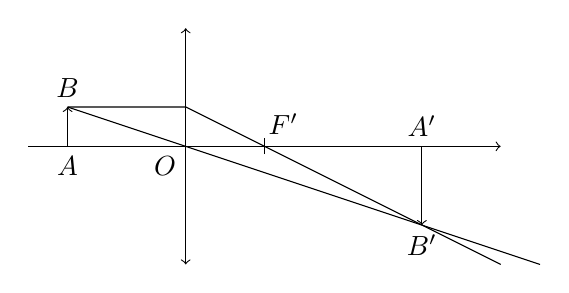
\begin{tikzpicture}
		\draw[->] (0,0) -- (2,0) node[below left]{$O$} -- (6,0);
		\draw[->] (.5,0) node[below]{$A$} -- ++(0,.5) node[above]{$B$};
		\draw[<->] (2,1.5) -- (2,-1.5);
		\draw (.5,.5) -- (6.5,-1.5);
		\draw (.5,.5) -- (2,.5) -- (6,-1.5);
		\draw (3,-.1) -- ++(0,.2) node[above right=-2pt]{$F'$};
		\draw[->] (5,0) node[above]{$A'$} -- (5,-1) node[below]{$B'$};
	\end{tikzpicture}
\end{minipage}
\par

On obtient ainsi la formule de conjugaison de Descartes: \fcolorbox{red}{white}{\( \dfrac{1}{\overline{OA'}} = \dfrac{1}{\overline{OA}} + \dfrac{1}{f'}\)}

\end{document}
